\section{~Wave Model Structure and Data Flow} \label{chapt:run}
\newcounters

\vsssub
\subsection{~Program design} \label{run:design}
\vssub

The core of \ws\ is the wave model subroutine, which can be
called by either a stand-alone program shell or any other program that
requires dynamically updated wave data. Two such programs are provided with
the \ws\ release (e.g., {\code ww3\_shel} and {\code ww3\_multi}). 
Auxiliary programs include a grid preprocessor {\code ww3\_grid}, a program to
generate artificial initial conditions {\code ww3\_strt}, generic program shells
for individual {\code ww3\_shel} or multi-grid {\code ww3\_multi} applications,
two input pre-processors ({\code ww3\_prep} and {\code ww3\_prnc}), and  
post-processors for gridded ({\code ww3\_outf} and {\code ww3\_ounf}) and point 
({\code ww3\_outp} and {\code ww3\_ounp}) output data.

In this section, note that file names will be identified by the {\file
file} type font, the contents of a file by the {\code code} type font and {\sc
fortran} program elements by the {\F fortran} type font. The main wave model 
subroutine is {\F w3wave}. Data files are identified with the
file extension {\file .ww3}, except in the multi-grid wave model {\file
ww3\_multi}, where the file extension identifies individual grids part of a chosen
multi-grid mosaic. For simplicity, the file extension {\file .ww3} will be used 
throughout this chapter.  

A relational diagram including the basic data flow is presented in 
Fig.~\ref{fig:run_elements}. The figure illustrates a typical workflow, as follows.
 The grid pre-processor {\code ww3\_grid} writes a model definition file {\file mod\_def.ww3} with
bottom and obstruction information and parameter values defining the physical
and numerical approaches. The wave model may have cold or hot starts. 
Hot starting requires a restart file {\file restart.ww3}, created either
by the wave model itself in a previous run, or by the initial conditions program {\code ww3\_strt}.
If a restart file is not available, the wave model will be initialized automatically.
If linear growth or spectral seeding is switch on, the model may start from a flat ocean ($H_s
= 0$), otherwise the initial conditions will consist of a parametric
fetch-limited spectrum based on the initial wind field (see the corresponding
option in the initial conditions program).  

The wave model routine ({\F
  w3wave}) optionally generates up to 9 restart files {\file
  restart{\em{n}}.ww3}, where {\file{\em{n}}} represents a single digit
integer number. For telescoping nest applications, the wave model also 
optionally reads boundary conditions from
the file {\file nest.ww3} and generates boundary conditions for consecutive
nested runs in {\file nest{\em{n}}.ww3}. The model furthermore dumps raw data to the
output files {\file out\_grd.ww3 }, {\file out\_pnt.ww3}, {\file track\_o.ww3}
and {\file partition.ww3} (gridded mean wave parameters, spectra at locations,
spectra along tracks, and partitioned wave data, respectively). The tracks
along which spectra are to be presented is defined in the file {\file
  track\_i.ww3}. Note that the wave model does not write to standard output,
because this would be inconvenient if \ws\ is part of an integrated
model. Instead, it maintains its own log file {\file log.ww3} and optionally a
test output files {\file test.ww3} for a shared memory version of the model,
or {\file test{\em{nnn}}.ww3} for distributed memory versions, where {\em nnn}
is the processor number starting with 1.  Finally, various output
post-processors are available (binary post-processing of raw gridded fields,
point output and track output files; NetCDF and GRIB(2) packing of wave data;
post-processing for later GrADS graphical processing of gridded and spectral
data). A more detailed description of all program elements and their input
files is given below. Note that the source codes of each routine are fully
documented. This documentation is an additional source of information about
\ws.

\setlength{\unitlength}{0.1mm}
\begin{figure}

\begin{picture}(1370,1080)(0,-1080)

\put(  50,  -80){\dashbox{5}(280,80)[c]{{\file grid data}}}
\put( 190,  -80){\vector(0,-1){60}}

\put(   0, -220){\framebox(380,80)[c]{grid preprocessor}}
\put( 190, -220){\vector(0,-1){60}}

\put(  50, -360){\dashbox{5}(280,80)[c]{{\file mod\_def.ww3}}}
\put( 190, -360){\vector(0,-1){380}}
\put( 190, -460){\vector(1,0){60}}
\put( 330, -320){\line(1,0){560}}
\put( 890, -320){\vector(1,1){100}}
\put( 890, -320){\line(1,-1){80}}
\put( 970, -400){\vector(0,-1){160}}

\put( 250, -500){\framebox(280,80)[c]{initial cond.}}
\put( 530, -460){\vector(1,0){60}}

\put( 590, -500){\dashbox{5}(280,80)[c]{{\file restart.ww3}}}
\put( 870, -500){\vector(1,-1){60}}

\put( 590, -640){\makebox(280,80)[c]{{\file restart.ww3}}}
\put( 590, -680){\makebox(280,80)[c]{{\file nest.ww3}}}
\put( 590, -680){\dashbox{5}(280,120)[c]{ }}

\put( 930, -640){\dashbox{10}(280,80)[c]{{\code wave model}}}
\put( 930, -600){\vector(-1,0){60}}
\put( 870, -600){\vector(1,0){60}}

\put( 590, -860){\makebox(280,80)[c]{{\file partition.ww3}}}
\put( 590, -780){\makebox(280,80)[c]{{\file out\_pnt.ww3}}}
\put( 590, -820){\makebox(280,80)[c]{{\file out\_grd.ww3}}}
\put( 590, -860){\dashbox{5}(280,170)[c]{ }}
\put( 970, -780){\vector(-1,0){100}}
\put( 590, -780){\vector(-1,0){60}}

\put( 970, -640){\vector(0,-1){240}}
\put( 830, -960){\makebox(280,80)[c]{{\file log.ww3}}}
\put( 830,-1000){\makebox(280,80)[c]{{\file test.ww3}}}
\put( 830,-1000){\dashbox{5}(280,120)[c]{ }}

\put(1170, -640){\vector(0,-1){100}}
\put(1170, -740){\vector(0,1){100}}
\put(1030, -820){\makebox(280,80)[c]{{\file track\_i.ww3}}}
\put(1030, -860){\makebox(280,80)[c]{{\file track\_o.ww3}}}
\put(1030, -860){\dashbox{5}(280,120)[c]{ }}

\put( 150, -820){\makebox(380,80)[c]{output}}
\put( 150, -860){\makebox(380,80)[c]{postprocessing}}
\put( 150, -860){\framebox(380,120)[c]{ }}

\put(1020, -560){\line(0,1){280}}
\put(1020, -280){\line(1,0){320}}
\put(1210, -620){\line(1,0){130}}
\put(1340, -620){\line(0,1){340}}
\put(1020, -370){\makebox(320,80)[c]{program}}
\put(1020, -410){\makebox(320,80)[c]{shell}}
\put(1020, -450){\makebox(320,80)[c]{or}}
\put(1020, -490){\makebox(320,80)[c]{integrated}}
\put(1020, -540){\makebox(320,80)[c]{program}}

\put(1040,  -80){\dashbox{5}(280,80)[0,0]{{\file input files}}}
\put(1170,  -80){\vector(0,-1){60}}

\put( 990, -220){\framebox(380,80)[c]{input preprocessor}}
\put(1170, -220){\vector(0,-1){60}}

{\scriptsize
\put(  50,-1010){\dashbox{5}(150,40)[0,0]{{\file file}}}
\put( 240,-1010){\dashbox{10}(150,40)[c]{{\code subrout.}}}
\put( 430,-1010){\framebox(150,40)[c]{program}}
\put( 140,-1050){\vector(1,0){60}}
\put( 220,-1070){\makebox(400,40)[l]{data transfer by file}}
\put(   0,-1090){\framebox(630,150){ }}                 }

\end{picture}

\caption{Basic program elements and data flow.}
\label{fig:run_elements}

\botline

\end{figure}


Files specific to \ws\ are opened by name within program subroutines. The unit
numbers, however, are defined by the user\footnote{~Except for {\file
ww3\_multi}.} within each {\file \.inp}, guaranteeing the largest possible 
flexibility for implementation in integrated models.

In addition to the wave model subroutine, an initialization routine and an interface
routine for data assimilation are provided. The routine includes a
generic interface that provides all necessary model components to perform full
spectral data assimilation. This routine is integrated into the generic wave
model shell, which is set up to perform time step managements for a wave model
with or without data assimilation. The shell also provides a simple yet
flexible way to provide the data assimilation scheme with various types of
data. Data assimilation has not yet been included in the multi-grid wave model
shell.

\vssub
\subsection{~The wave model routines} \label{sec:core}
\vssub

The wave model driver is a subroutine within the \ws\ framework package. 
To run the model driver subroutine, a program shell is needed. 
\ws\ is provided with a simple stand-alone shell as
will be discussed in \para\ref{sec:ww3shel}, and with a more complex
multi-grid model shell as will be discussed in \para\ref{sec:ww3multi}. The
present section concentrates on the wave model driver subroutines.

The wave model initialization routine {\F w3init} performs model
initialization for a single wave model grid. This includes setting up part of
the I/O system by defining unit numbers, initializing internal time
management, processing the model definition file ({\file mod\_def.ww3}),
processing initial conditions ({\file restart.ww3}), preparing model output,
and calculating grid-dependent parameters. If the model is compiled for an
\mpi\ environment, all necessary communication for both calculations and
output are determined and initialized (the model uses persistent \mpi\
communication throughout).

The wave model routine {\F w3wave} can be called any number of times to
propagate the wave field for a single grid in time after the initialization
has taken place. After some initial checks, the subroutine interpolates winds
and currents, updates ice concentrations and water levels, propagates the wave
field, and applies the selected source terms for a number of time steps. The
internal time step is defined by the interval for which the calculations are
to be performed, and by the requested output times. At the end of the
calculations, the routine provides the calling program with the requested
fields of wave data. A documentation of the interface of {\F w3wave} can be
found in the source code ({\file w3wavemd.ftn}).

\begin{figure}
{\small \begin{verbatim}
                                    |    input    |     output    |
                                    |-------------|---------------|
  step | pass |    date      time   | b w l c i d | g p t r b f c |
-------|------|---------------------|-------------|---------------|
    0  |   1  | 1968/06/06 00:00:00 |   F         | X X           |
    8  |   1  |            02:00:00 |             |   X           |
   12  |   1  |            03:00:00 |             | X             |
   16  |   1  |            04:00:00 |             |   X           |
   24  |   1  |            06:00:00 |   X         | X X           |
   32  |   2  |            08:00:00 |             |   X           |
   36  |   2  |            09:00:00 |             | L             |
   40  |   2  |            10:00:00 |             |   X           |
   48  |   2  |            12:00:00 |   X       X |   L   L       |
-------+------+---------------------+-------------+---------------+ 
\end{verbatim} }
\caption{Example action table from file {\file log.ww3}.} \label{fig:log}
\botline
\end{figure}
 

Apart from the raw data files as described above, the program maintains a log
file {\file log.ww3}. This file is opened by {\F w3init} (contained in {\F
  w3wave} in {\file w3wavemd.ftn}), which writes some self-explanatory header
information to this file. Each consecutive call to {\F w3wave} adds several
lines to an `action table' in this log file as is shown in
Fig.~\ref{fig:log}. The column identified as `step' shows the discrete time
step considered. The column identified as `pass' identifies the sequence
number of the call to {\F w3wave}; i.e., 3 identifies that this action took
place in the third call to {\F w3wave}. The third column shows the ending time
of the time step. In the input and output columns the corresponding actions of
the model are shown. A {\tt X} identifies that the input has been updated, or
that the output has been performed. A {\tt F} indicates a first field read,
and an {\tt L} identifies the last output. The seven input columns identify
boundary conditions ({\tt b}), wind fields ({\tt w}), water levels ({\tt l}),
current fields ({\tt c}), ice concentrations ({\tt i}), and data for
assimilation ({\tt d}), respectively. Note that data assimilation takes place
at the end of the time step after the wave routine call. The seven output
columns identify gridded output ({\tt g}), point output ({\tt p}), output
along tracks ({\tt t}), restart files ({\tt r}), boundary data ({\tt b}), and
partitioned spectral data ({\tt f}), and output for coupling ({\tt c}),
respectively.

For the multi-grid wave model \citep[][{\file ww3\_multi}]{tol:OMOD08b} a set
of routines is build around the basic wave model routines. The three main
routines are the initialization routine {\F wminit}, a time stepping routine
{\F wmwave} and a finalization routine {\F wmfinl}, with similar functions as
the routines for a single grid as described above. Note that the raw input and
output files are generated for separate grid in the mosaic, and are identified
by replacing the standard file extension '{\file .ww3}' with a unique
identifier for each individual grid as chosen by the user in the 
{\file ww3\_grid.inp} file. Log files are maintained for each individual grid, 
as well as an overall log file {\file log.mww3}.

\vssub
\subsection{~The data assimilation interface} \label{sec:das}
\vssub

As discussed above, the wave model subroutine is supplemented with a data
assimilation interface routine ({\F w3wdas} in {\file w3wdasmd.ftn}). This
routine is integrated in the stand-alone shell (see \para\ref{sec:ww3shel}) to
provide time step management of a combined wave model / data assimilation
scheme. It has not yet been integrated in the multi-grid model driver,
although it is accounted for in the multi-grid model management
algorithm. 

In this a fairly simple approach is assumed where data assimilation
is performed at selected times, while the wave model marches forward in
time. In the setup of the shell, the data assimilation is performed after the
model has reached the target time, but has not yet produced output. After the
data assimilation is performed, the wave model routine is called again only to
generate output as requested. Thus, the wave model output for a given time
will include the effects of data assimilation for that specific target time.

The generic program shell also processes several types of data to be
assimilated, and passes it on to the data assimilation interface routine. All
data needs to be preprocessed using the wave model input preprocessor (see
\para\ref{sec:ww3prep}), and will be recognized by the generic shell by file
name. Presently, up to three different data files can be used. Tentatively,
these could be mean wave parameters, one dimensional spectral data, and two
dimensional spectral data, respectively. This is, however, not hardwired to
the model and in fact needs to be defined by the user.

Presently, no data assimilation packages are available. Therefore, user supplied 
data assimilation schemes are required, and may be included in the wave model 
using the interface routine ({\F w3wdas} in {\file w3wdasmd.ftn}), the documentation 
of which should be sufficient for the necessary programming. Details on how to add 
user supplied software to the \ws\ compilation system can be found in the following
chapter. Although NCEP is presently working on wave data assimilation techniques, 
 there are no plans to distribute wave data assimilation software as part of the 
\ws\ package.

\vsssub
\subsubsection{~Auxiliary programs} \label{sec:aux_mod}
\vsssub

\vspace{\baselineskip}
\noindent
\ww\ has several auxiliary pre- and post-processors, and two wave model shells
(see \para\ref{sec:auxprog}). These auxiliary programs and some additional routines
are stored in the following files. Generally, subroutines used only by the
programs are stored as internal subroutines with the main program. There is no
need for using the module structure in this case. The exception is an
additional module {\file w3fldsmd.ftn} which deals with the data flow of input
fields for the wave model between the field pre-processor and the stand-alone
model shell. The latter module does not have any explicit \ws\ dependencies,
and can therefore be integrated in any custom data pre-processor.

% fig:prepro

% \newcommand{\la }{  10}
\newcommand{\lab}{ 110}
\newcommand{\lb }{ 160}
\newcommand{\ca }{ 510}
\newcommand{\cab}{ 610}
\newcommand{\cb }{ 660}
\newcommand{\ra }{1010}
\newcommand{\rab}{1110}
\newcommand{\rb }{1160}
\setlength{\unitlength}{0.1mm}

\begin{figure}
\begin{picture}(1370,500)(0,-400)

\subr{\la}{   0}{w3grid}
\subr{\lb}{-100}{readnl}
\subr{\lb}{-200}{distab}
\subr{\lb}{-300}{inptab}
\subr{\lb}{-400}{w3iogr}
\put(\lab,-370){\line(0,1){370}}
\multiput(\lab,-370)(0,100){4}{\line(1,0){50}}

\subr{\ca}{   0}{w3strt}
\subr{\cb}{-100}{w3iogr}
\subr{\cb}{-200}{w3iors}
\put(\cab,-170){\line(0,1){170}}
\multiput(\cab,-170)(0,100){2}{\line(1,0){50}}

\subr{\ra}{   0}{w3prep}
\subr{\rb}{-100}{w3iogr}
\subr{\rb}{-200}{w3fldp}
\subr{\rb}{-300}{w3fldo}
\subr{\rb}{-400}{w3fldg}
\put(\rab,-370){\line(0,1){370}}
\multiput(\rab,-370)(0,100){4}{\line(1,0){50}}

\end{picture}

\caption{Subroutine structure of pre-processors}
\label{fig:prepro}

\botline
\end{figure}


\vspace{\baselineskip} 
\noindent
Input data file management module \hfill {\file w3fldsmd.ftn}

\begin{flisti}
\fit{w3fldo}{Opening and checking of data files for {\F w3shel}.}
\fit{w3fldg}{Reading and writing of data files for {\F w3shel} (model input).}
\fit{w3fldd}{Reading and writing of data files for {\F w3shel} (data assimilation).}
\fit{w3fldp}{Prepare interpolation of input fields from arbitrary grids.}
\fit{w3fldh}{Management of homogeneous input fields in {\F w3shel}.}
\fit{w3fldm}{Process moving grid data in {\F w3shel}.}
\end{flisti}

\noindent
Grid pre-processing program \hfill {\file ww3\_grid.ftn}

\begin{flisti}
\fit{w3grid}{The grid preprocessor.}
\fit{readnl}{Reading {\F namelist} input (internal).}
\end{flisti}

\noindent
Initial conditions program \hfill {\file ww3\_strt.ftn}

\begin{flisti}
\fit{w3strt}{The initial conditions program.}
\end{flisti}

\noindent
Boundary conditions program \hfill {\file ww3\_bound.ftn}

\noindent
Boundary conditions program (NetCDF) \hfill {\file ww3\_bounc.ftn}

\begin{flisti}
\fit{w3bound}{The boundary conditions program (NetCDF).}
\end{flisti}

\noindent
Input field pre-processing program \hfill {\file ww3\_prep.ftn}

\noindent
Input field pre-processing program from NetCDF files \hfill {\file ww3\_prnc.ftn}

\begin{flisti}
\fit{w3prep}{Pre-processor for the input fields for the generic shell.}
\end{flisti}

\noindent
Tide pre-processing program \hfill {\file ww3\_prtide.ftn}

\begin{flisti}
\fit{w3prtide}{Pre-processor for tides.}
\end{flisti}

\noindent
Restart file pre-processing program \hfill {\file ww3\_uprstr.ftn}

\begin{flisti}
\fit{w3uprstr}{The restart file preprocessor.}
\fit{readnl}{Reading {\F namelist} input (internal).}
\end{flisti}

\noindent
Generic wave model program \hfill {\file ww3\_shel.ftn}

\begin{flisti}
\fit{w3shel}{The generic program shell.}
\end{flisti}

% fig:shell

% \setlength{\unitlength}{0.1mm}

\begin{figure}
\begin{picture}(1370,700)(0,-600)

\subr{410}{   0}{w3shel}
\subr{560}{-100}{w3fldo}
\subr{560}{-200}{w3wave}
\subc{810}{-200}{Fig. \ref{fig:w3wave}}
\subr{560}{-300}{w3wdas}
\subr{560}{-400}{w3fldh}
\subr{560}{-500}{w3fldg}
\subr{560}{-600}{w3fldm}
\put(510,-580){\line(0,1){570}}
\multiput(510,-580)(0,100){6}{\line(1,0){50}}
\multiput(760,-170)(0,200){1}{\line(1,0){50}}

\end{picture}

\caption{Subroutine structure for the generic program shell.}
\label{fig:shell}

\botline
\end{figure}


\noindent
Grid splitting for {\file ww3\_multi} \hfill {\file ww3\_gspl.ftn}

\begin{flisti}
\fit{w3gspl}{The grid splitting program.}
\fit{grinfo, grtrim grfill, grlost, grsqrg, grsngl, grsepa, grfsml, grfrlg, gr1grd}{}
\fit{      }{\vspace{-\baselineskip} Routines to incrementally adjust individual grids.}
\end{flisti}

\noindent
Generic wave model program \hfill {\file ww3\_multi.ftn}

\begin{flisti}
\fit{w3mlti}{The multi-grid program shell.}
\end{flisti}

\noindent
Grid output integration for {\file ww3\_multi} \hfill {\file ww3\_gint.ftn}

\begin{flisti}
\fit{w3gint}{The post-processing program for integrating gridded
                    fields of mean wave parameters.}
\fit{w3exgi}{Actual output routine (internal).}
\end{flisti}

\noindent
Gridded data post-processing program \hfill {\file ww3\_outf.ftn}

\begin{flisti}
\fit{w3outf}{The post-processing program for gridded
                    fields of mean wave parameters.}
\fit{w3exgo}{Actual output routine (internal).}
\end{flisti}

\pb \noindent
Gridded data post-processing program (NetCDF) \hfill {\file ww3\_ounf.ftn}

\begin{flisti}
\fit{w3ounf}{The post-processing program for gridded
             fields of mean wave parameters, using NetCDF3 or
             NetCDF4 libraries for Fortran90.}
\fit{w3crnc}{Creation of NetCDF files, definition of dimensions and header data.}
\fit{w3exnc}{Actual output routine (internal).}
\end{flisti}

\noindent
Gridded data post-processing program (GrADS) \hfill {\file gx\_outf.ftn}

\begin{flisti}
\fit{gxoutf}{The post-processing program for converting gridded
             fields of mean wave parameters to input files for GrADS.}
\fit{gxexgo}{Actual output routine (internal).}
\end{flisti}

\noindent
Gridded data post-processing program (GRIB) \hfill {\file ww3\_grib.ftn}

\begin{flisti}
\fit{w3grib}{The post-processing program for generating GRIB files.}
\fit{w3exgb}{Actual output routine (internal).}
\end{flisti}

% fig:post

% \setlength{\unitlength}{0.1mm}

\begin{figure}
\begin{picture}(1370,600)(0,-500)

\subr{ 50}{   0}{w3outf}
\subr{200}{-100}{w3iogr}
\subr{200}{-200}{w3iogo}
\subr{200}{-300}{w3exgo}
\put(150,-270){\line(0,1){270}}
\multiput(150,-270)(0,100){3}{\line(1,0){50}}

\subr{550}{   0}{w3outp}
\subr{700}{-100}{w3iogr}
\subr{700}{-200}{w3iopo}
\subr{700}{-300}{w3expo}
\put(650,-270){\line(0,1){270}}
\multiput(650,-270)(0,100){3}{\line(1,0){50}}

\subn{1000}{-100}{w3spr}
\subn{1000}{-200}{w3sin}
\subn{1000}{-300}{w3snl}
\subn{1000}{-400}{w3sds}
\subn{1000}{-500}{w3sbt}
\put(950,-270){\line(-1,0){50}}
\put(950,-470){\line(0,1){400}}
\multiput(950,-470)(0,100){5}{\line(1,0){50}}

\end{picture}

\caption{Subroutine structure for the postprocessors. The structure of the GRIB postprocessor is similar to {\F w3outf}, replacing {\F w3outf} and {\F w3exgo} with {\F w3grib} and {\F w3exgb}, respectively. The structure of the GrADS postprocessors is similar, replacing {\F w3outf}, {\F w3outp}, {\F w3exgo} and {\F w3expo} with {\F gxoutf}, {\F gxoutp}, {\F gxexgo} and {\F gxexpo}, respectively}
\label{fig:post}

\botline
\end{figure}


\noindent
Point post-processing program \hfill {\file ww3\_outp.ftn}

\begin{flisti}
\fit{w3outp}{The post-processing program output at selected locations.}
\fit{w3expo}{Actual output routine (internal).}
\end{flisti}

\noindent
Point post-processing program \hfill {\file ww3\_ounp.ftn}

\begin{flisti}
\fit{w3ounp}{The post-processing program output at selected locations using NetCDF.}
\fit{w3crnc}{Creation of NetCDF files, definition of dimensions and header data.}
\fit{w3exnc}{Actual output routine (internal).}
\end{flisti}

\noindent
Point post-processing program (GrADS) \hfill {\file gx\_outp.ftn}

\begin{flisti}
\fit{gxoutp}{The post-processing program for converting output
             at selected locations to input files for GrADS.}
\fit{gxexpo}{Actual output routine (internal).}
\end{flisti}

\noindent
Track output post-processing program \hfill {\file ww3\_trck.ftn}

\begin{flisti}
\fit{w3trck}{Converting unformatted direct access track
             output file to integer-packed formatted file.}
\end{flisti}

\noindent
Track output post-processing program \hfill {\file ww3\_trnc.ftn}

\begin{flisti}
\fit{w3trck}{Converting unformatted direct access track
	     output file to NetCDF file.}
\fit{w3crnc}{Creation of NetCDF files, definition of dimensions and header data.}
\fit{w3exnc}{Actual output routine (internal).}
\end{flisti}

\noindent
Wave field tracking post-processing program \hfill {\file ww3\_systrk.ftn}

\begin{flisti}
\fit{w3systrk}{Tracking wave fields in space and time.}
\end{flisti}

\vsssub
\subsubsection{The grid preprocessor} \label{sub:ww3grid}
\vsssub

\proddefH{ww3\_grid}{w3grid}{ww3\_grid.ftn}
\proddeff{Input}{ww3\_grid.nml}{Namelist configuration file.}{10} (App.~\ref{sec:config012})
\proddefa{ww3\_grid.inp}{Traditional configuration file.}{10} (App.~\ref{sec:config011})
\proddefa{'grid file' \opt}{File with bottom depths.}{user}
\proddefa{'obstr. file' \opt}{File with sub-grid obstructions. }{user}
\proddefa{'mask file' \opt}{File with grid mask. }{user}
\proddeff{Output}{standard out}{Formatted output of program.}{6}
\proddefa{mod\_def.ww3}{Model definition file in \ws\ format.}{20}
\proddefa{mask.ww3 \opt}{Land-sea mask file (switch {\F o2}a).}{20}
\proddeff{Scratch}{ww3\_grid.scratch}{Formatted scratch file.}{90}

\vspace{\baselineskip} \noindent
Note that bottom and obstruction data may be in same file.

\pb

\begin{footnotesize}
\begin{verbatim}
$ -------------------------------------------------------------------- $
$ WAVEWATCH III Initial conditions input file                          $
$--------------------------------------------------------------------- $
$ type of initial field ITYPE .
$
    1
$
$ ITYPE = 1 ---------------------------------------------------------- $
$ Gaussian in frequency and space, cos type in direction.
$ - fp and spread (Hz), mean direction (degr., oceanographic
$    convention) and cosine power, Xm and spread (degr. or m) Ym and
$    spread (degr. or m), Hmax (m) (Example for lon-lat grid in degr.).
$
$   0.10  0.01  270. 2  1. 0.5 1. 0.5 2.5
    0.10  0.01  270. 2  0. 1000. 1. 1000. 2.5
$   0.10  0.01  270. 2  0. 1000. 1. 1000. 0.01
$   0.10  0.01  270. 2  0. 1000. 1. 1000. 0.
$
$ ITYPE = 2 ---------------------------------------------------------- $
$ JONSWAP spectrum with Hasselmann et al. (1980) direct. distribution.
$ - alfa, peak freq. (Hz), mean direction (degr., oceanographical
$   convention), gamma, sigA, sigB, Xm and spread (degr. or m) Ym and
$   spread (degr. or m)  (Example for lon-lat grid in degr.).
$   alfa, sigA, sigB give default values if less than or equal to 0.
$
$   0.0081  0.1  270.  1.0 0. 0. 1. 100. 1. 100.
$
$ ITYPE = 3 ---------------------------------------------------------- $
$ Fetch-limited JONSWAP
$ - No additional data, the local spectrum is calculated using the
$   local wind speed and direction, using the spatial grid size as
$   fetch, and assuring that the spectrum is within the discrete
$   frequency range.
$
$ ITYPE = 4 ---------------------------------------------------------- $
$ User-defined spectrum
$ - Scale factor., defaults to 1 if less than or equal 0.
$ - Spectrum F(f,theta) (single read statement)
$
$ -0.1
$  0 0 0 0 0 0 0 0 0 0 0 0 0 0 0 0 0 0 0 0 0 0 0 0 0
$  0 1 1 1 0 0 0 0 0 0 0 0 0 0 0 0 0 0 0 0 0 0 0 0 0
$  0 1 4 2 1 0 0 0 0 0 0 0 0 0 0 0 0 0 0 0 0 0 0 0 0
$  0 0 1 1 0 0 0 0 0 0 0 0 0 0 0 0 0 0 0 0 0 0 0 0 0
$  0 0 0 0 0 0 0 0 0 0 0 0 0 0 0 0 0 0 0 0 0 0 0 0 0
$  0 0 0 0 0 0 0 0 0 0 0 0 0 0 0 0 0 0 0 0 0 0 0 0 0
$  0 0 0 0 0 0 0 0 0 0 0 0 0 0 0 0 0 0 0 0 0 0 0 0 0
$  0 0 0 0 0 0 0 0 0 0 0 0 0 0 0 0 0 0 0 0 0 0 0 0 0
$  0 0 0 0 0 0 0 0 0 0 0 0 0 0 0 0 0 0 0 0 0 0 0 0 0
$  0 0 0 0 0 0 0 0 0 0 0 0 0 0 0 0 0 0 0 0 0 0 0 0 0
$  0 0 0 0 0 0 0 0 0 0 0 1 1 1 1 0 0 0 0 0 0 0 0 0 0
$  0 0 0 0 0 0 0 0 0 0 1 2 3 2 1 1 0 0 0 0 0 0 0 0 0
$  0 0 0 0 0 0 0 0 0 1 3 9 7 5 3 2 1 0 0 0 0 0 0 0 0
$  0 0 0 0 0 0 0 0 0 0 1 3 4 3 2 1 0 0 0 0 0 0 0 0 0
$  0 0 0 0 0 0 0 0 0 0 0 1 1 1 1 0 0 0 0 0 0 0 0 0 0
$  0 0 0 0 0 0 0 0 0 0 0 0 0 0 0 0 0 0 0 0 0 0 0 0 0
$  0 0 0 0 0 0 0 0 0 0 0 0 0 0 0 0 0 0 0 0 0 0 0 0 0
$  0 0 0 0 0 0 0 0 0 0 0 0 0 0 0 0 0 0 0 0 0 0 0 0 0
$  0 0 0 0 0 0 0 0 0 0 0 0 0 0 0 0 0 0 0 0 0 0 0 0 0
$  0 0 0 0 0 0 0 0 0 0 0 0 0 0 0 0 0 0 0 0 0 0 0 0 0
$  0 0 0 0 0 0 0 0 0 0 0 0 0 0 0 0 0 0 0 0 0 0 0 0 0
$  0 0 0 0 0 0 0 0 0 0 0 0 0 0 0 0 0 0 0 0 0 0 0 0 0
$  0 0 0 0 0 0 0 0 0 0 0 0 0 0 0 0 0 0 0 0 0 0 0 0 0
$  0 0 0 0 0 0 0 0 0 0 0 0 0 0 0 0 0 0 0 0 0 0 0 0 0
$
$ ITYPE = 5 ---------------------------------------------------------- $
$ Starting from calm conditions.
$ - No additional data.
$
$ -------------------------------------------------------------------- $
$ End of input file                                                    $
$ -------------------------------------------------------------------- $
\end{verbatim}
\end{footnotesize}

\vsssub
\subsubsection{The boundary conditions program} \label{sub:ww3bound}
\vsssub

\proddefH{ww3\_bound}{w3bound}{ww3\_bound.ftn}
\proddeff{Input}{ww3\_bound.inp}{Traditional configuration file.}{10} (App.~\ref{sec:config031})
\proddefa{mod\_def.ww3}{Model definition file.}{20}
\proddefa{'spectra file' \opt}{File(s) with wave spectra.}{user}
\proddeff{Output}{standard out}{Formatted output of program.}{6}
\proddefa{nest.ww3}{Boundary conditions file.}{33}

\vspace{\baselineskip} \noindent
Note: When using this program to produce boundary inputs for a model formulated on rotated pole grid, the input spectra are always assumed to be formulated on a standard pole.

\pb

\begin{footnotesize}
\begin{verbatim}
$ -------------------------------------------------------------------- $
$ WAVEWATCH III NetCDF boundary input processing                       $
$--------------------------------------------------------------------- $
$
$ Boundary option: READ or WRITE
$
 WRITE 
$
$ Interpolation method: 1: nearest
$                       2: linear interpolation
 2 
$ Verbose (0, 1, 2)
1
$
$ List of spectra files. These NetCDF files use the WAVEWATCH III
$ format as described in the ww3_ounp.inp file. The files are 
$ defined relative to the directory in which the program is run.
$
SPECTRA_NC/ww3.62163_spec.nc
SPECTRA_NC/ww3.62069_spec.nc
'STOPSTRING'
$
$ -------------------------------------------------------------------- $
$ End of input file                                                    $
$ -------------------------------------------------------------------- $
\end{verbatim}
\end{footnotesize}

\vsssub
\subsubsection{The input field preprocessor } \label{sec:ww3prep}
\vsssub

\proddefH{ww3\_prep}{w3prep}{ww3\_prep.ftn}
\proddeff{Input}{ww3\_prep.inp}{Traditional configuration file.}{10} (App.~\ref{sec:config051})
\proddefa{mod\_def.ww3}{Model definition file.}{11}
\proddefa{'user input'\opt}{See example below.}{user}
\proddeff{Output}{standard out}{Formatted output of program.}{6}
\proddefa{level.ww3\opt}{Water levels file.}{12}
\proddefa{current.ww3\opt}{Current fields file.}{12}
\proddefa{wind.ww3\opt}{Wind fields file.}{12}
\proddefa{ice.ww3\opt}{Ice fields file.}{12}
\proddefa{data0.ww3\opt}{Assimilation data (`mean').}{12}
\proddefa{data1.ww3\opt}{Assimilation data (`1-D spectra').}{12}
\proddefa{data2.ww3\opt}{Assimilation data (`2-D spectra').}{12}

\vspace{\baselineskip} 
\vspace{\baselineskip} 

\noindent 
Note that the optional output files are specific to {\file ww3\_shel} and
{\file ww3\_multi}, but are not processed by the actual wave model
routines. These files are consequently not needed if the wave model routines
are used in a different shell or in an integrated program. However, the
routines reading and writing these files are system-independent and could
therefore be used in customized applications of the basic wave model. The
reading and writing of these files is performed by the subroutine {\F w3fldg}
({\file w3fldsmd.ftn}). For additional documentation and file formats
reference if made to this routine.
\pb

\begin{footnotesize}
\begin{verbatim}
$ -------------------------------------------------------------------- $
$ WAVEWATCH III Field preprocessor input file                          $
$ -------------------------------------------------------------------- $
$ Major types of field and time flag
$   Field types  :  IC1   Ice thickness.
$                   IC5   Ice floe mean diameter.
$                   ICE   Ice concentrations.
$                   ISI   Icebergs and sea ice.
$                   LEV   Water levels.
$                   WND   Winds.
$                   WNS   Winds (including air-sea temp. dif.)
$                   CUR   Currents.
$                   DAT   Data for assimilation.
$
$   Format types :  AI    Transfer field 'as is'. (ITYPE 1)
$                   LL    Field defined on regular longitude-latitude
$                         or Cartesian grid. (ITYPE 2)
$   Format types :  AT    Transfer field 'as is', performs tidal 
$                         analysis on the time series (ITYPE 6)
$                         When using AT, another line should be added
$                         with the choice of tidal constituents:
$                         FAST or VFAST or a list: e.g. 'M2 S2'
$
$        - Format type not used for field type 'DAT'.
$
$   Time flag    : If true, time is included in file.
$   Header flag  : If true, header is added to file.
$                  (necessary for reading, FALSE is used only for
$                   incremental generation of a data file.)
$
  'WND' 'LL' T T
$
$ Name of spatial dimensions------------------------------------------ $
$ NB: time dimension is expected to be called 'time' and must respect 
$     Julian or Gregorian calendar with leap day.
$
 longitude latitude
$
$ Variables to use --------------------------------------------------- $
$
  U V
$
$ Additional time input ---------------------------------------------- $
$ If time flag is .FALSE., give time of field in yyyymmdd hhmmss format.
$
$   19680606 053000
$
$ Define data files -------------------------------------------------- $
$ The input line identifies the filename using for the forcing field.
$
  'wind.nc'
$
$ -------------------------------------------------------------------- $
$ End of input file                                                    $
$ -------------------------------------------------------------------- $
\end{verbatim}
\end{footnotesize}

\vsssub
\subsubsection{The tide prediction program} \label{sub:ww3prtide}
\vsssub

\proddefH{ww3\_prtide}{w3tide}{ww3\_prtide.ftn}
\proddeff{Input}{ww3\_prtide.inp}{Traditional configuration file.}{10} (App.~\ref{sec:config071})
\proddefa{mod\_def.ww3}{Model definition file.}{20}
\proddefa{current.ww3\_tide or level.ww3\_tide}{File with tidal constituents.}{user}
\proddeff{Output}{standard out}{Formatted output of program.}{6}
\proddefa{current.ww3 or level.ww3}{Level or current forcing.}{33}

\vspace{\baselineskip} 
\vspace{\baselineskip} 
\noindent 
The user-provided file current.ww3\_tide or level.ww3\_tide is a binary file
that can be obtained by running ww3\_prnc with the 'AT' option and then
renaming the resulting file current.ww3 or level.ww3 into current.ww3\_tide or
level.ww3\_tide . The choice of tidal constituents used for the tidal
prediction can be a subset of the ones present in these files or all of them.

Because of wetting and drying or grid mismatches, the tidal constituents may
be erroneous or absent for some of the \ws\ nodes. The erroneous ones can be
detected using a maximum amplitude on particular components. When the
amplitudes exceeds these maxima, then the tidal constituents are extrapolated
from the nearest nodes. This feature has only been tested on triangular
meshes.

\pb

\vsssub
\subsubsection{The generic shell} \label{sec:ww3shel}
\vsssub

\proddefH{ww3\_shel}{w3shel}{ww3\_shel.ftn}
\proddeff{Input}{ww3\_shel.nml}{Namelist configuration file.}{10} (App.~\ref{sec:config082})
\proddefa{ww3\_shel.inp}{Traditional configuration file.}{10} (App.~\ref{sec:config081})
\proddefa{mod\_def.ww3}{Model definition file.}{30}
\proddefa{restart.ww3}{Restart file.}{30}
\proddefa{nest.ww3\opt}{Boundary conditions file.}{33}
\proddefa{level.ww3\opt}{Water levels file.}{11}
\proddefa{current.ww3\opt}{Current fields file.}{12}
\proddefa{wind.ww3\opt}{Wind fields file.}{13}
\proddefa{ice.ww3\opt}{Ice fields file.}{14}
\proddefa{data0.ww3\opt}{Assimilation data.}{15}
\proddefa{data1.ww3\opt}{Assimilation data.}{16}
\proddefa{data2.ww3\opt}{Assimilation data.}{17}
\proddefa{track\_i.ww3\opt}{Output track information.}{22}
\proddeff{Output}{standard out}{Formatted output of program.}{6}
\proddefa{log.ww3}{Output log of wave model (see \para\ref{sec:core}).}{20}
\proddefa{test.ww3\opt}{Test output of wave model.}{6/21}
\proddefa{restart{\sl{n}}.ww3\opt}{Restart file(s).}{30}
\proddefa{nest{\sl{n}}.ww3\opt}{Nesting file(s).}{34-42}
\proddefa{out\_grd.ww3\opt}{Raw output of gridded fields.}{31}
\proddefa{out\_pnt.ww3\opt}{Raw output of spectra.}{32}
\proddefa{track\_o.ww3\opt}{Raw output of spectra along tracks.}{23}
\proddeff{Scratch}{ww3\_shel.scratch}{Formatted scratch file.}{90}

\pb

\begin{footnotesize}
\begin{verbatim}
$ -------------------------------------------------------------------- $
$ WAVEWATCH III Grid splitting input file                              $
$ -------------------------------------------------------------------- $
$ Grid identifier (file extension for mod_def file of grid to be split)
$
  'glo_2d'
$
$ Number of sub-grids to be created, maximum number of iterations,
$ target grid point count std in percent. user defined halo extension
$ (default should be 2, used because of inconsistencies between halo
$ computation in this code and in the main wave model code). Increase
$ the latter number if ww3_multi fails on halo overlaps between 
$ equally ranked grids.
$
  12  250  0.75  2
$
$ IDLA, IDFM, scale and RFORM for bottom, obstruction and mask files.
$ Note that the third file is integers. Suggest IDFM = 1 and IDLA = 1
$
   3   2   1.0   '(12F11.3)'
   3   2   1.0   '(26F5.2)'
   3   2   1     '(66I2)'
$
$ lowest and highest fraction of communicator to be used for grid.
$ and flag for running grids side-by-side inside fraction
$  F: for test purposes only, defeats most reasons for splitting
$  T: normal operations
$
   0.4  1.  F
$ -------------------------------------------------------------------- $
$ End of input file                                                    $
$ -------------------------------------------------------------------- $
\end{verbatim}
\end{footnotesize}

\begin{footnotesize}
\begin{verbatim}
$ -------------------------------------------------------------------- $
$ WAVEWATCH III multi-grid model driver input file                     $
$ -------------------------------------------------------------------- $
$
$ *******************************************************************
$ *** NOTE : This is an example file from the mww3_test_05 script ***
$ ***        Unlike other input example files this one CANNOT     ***
$ ***        be run as an independent interactive run             ***
$ *******************************************************************
$
$ The first input line sets up the general multi-grid model definition
$ by defining the following six parameters :
$
$   1) Number of wave model grids.                          ( NRGRD )
$   2) Number of grids defining input fields.               ( NRINP )
$   3) Flag for using unified point output file.           ( UNIPTS )
$   4) Output server type as in ww3_shel.inp
$   5) Flag for dedicated process for unified point output.
$   6) Flag for grids sharing dedicated output processes.
$
  3 1 T 1 T T
$
$ -------------------------------------------------------------------- $
$ If there are input data grids defined ( NRINP > 0 ), then these
$ grids are defined first. These grids are defined as if they are wave
$ model grids using the file mod_def.MODID. Each grid is defined on
$ a separate input line with MODID, and eight input flags identifying
$ the presence of 1) water levels 2) currents 3) winds 4) ice and
$ 5-7) assimilation data as in the file ww3_shel.inp.
$
  'input' F F T F F F F
$
$ In this example, we need the file mod_def.input to define the grid
$ and the file wind.input to provide the corresponding wind data.
$
$ -------------------------------------------------------------------- $
$ If all point output is gathered in a unified point output file
$ ( UNIPTS = .TRUE. ), then the output spectral grid needs to be 
$ defined. This information is taken from a wave model grid, and only
$ the spectral definitions from this grid are relevant. Define the
$ name of this grid here
$
  'points'
$
$ In this example, we need the file mod_def.points to define the
$ spectral output grid, and the point output will be written to the
$ file out_pnt.points
$
$ -------------------------------------------------------------------- $
$ Now each actual wave model grid is defined using 13 parameters to be
$ read from a single line in the file. Each line contains the following
$ parameters
$     1)   Define the grid with the extension of the mod_def file.
$    2-8)  Define the inputs used by the grids with 8 keywords 
$          corresponding to the 8 flags defining the input in the
$          input files. Valid keywords are:
$            'no'      : This input is not used.
$            'native'  : This grid has its own input files, e.g. grid
$                        grdX (mod_def.grdX) uses ice.grdX.
$            'MODID'   : Take input from the grid identified by 
$                        MODID. In the example below, all grids get
$                        their wind from wind.input (mod_def.input).
$     9)   Rank number of grid (internally sorted and reassigned).
$    10)   Group number (internally reassigned so that different
$          ranks result in different group numbers.
$   11-12) Define fraction of communicator (processes) used for this
$          grid. '0.00 1.00' is appropriate in many cases. Partial 
$          fractions, i.e. settings other than '0.00 1.00', are 
$          intended for equal rank grids, to improve scaling. The 
$          commented example provided here (partial fractions with
$          non-equal rank) is not generally recommended.
$    13)   Flag identifying dumping of boundary data used by this
$          grid. If true, the file nest.MODID is generated.
$
  'grd1'  'no' 'no' 'input' 'no' 'no' 'no' 'no'   1  1  0.00 1.00  F
  'grd2'  'no' 'no' 'input' 'no' 'no' 'no' 'no'   2  1  0.00 1.00  F
  'grd3'  'no' 'no' 'input' 'no' 'no' 'no' 'no'   3  1  0.00 1.00  F
$ 'grd1'  'no' 'no' 'input' 'no' 'no' 'no' 'no'   1  1  0.00 0.50  F
$ 'grd2'  'no' 'no' 'input' 'no' 'no' 'no' 'no'   2  1  0.25 0.75  F
$ 'grd3'  'no' 'no' 'input' 'no' 'no' 'no' 'no'   3  1  0.50 1.00  F
$
$ In this example three grids are used requiring the files
$ mod_def.grdN. All files get their winds from the grid 'input'
$ defined by mod_def.input, and no other inputs are used. In the lines
$ that are commented out, each grid runs on a part of the pool of
$ processes assigned to the computation.
$
$ Limitations relevant to irregular (curvilinear) grids:
$   1) Equal rank is not supported when one or more is an irregular
$       grid. Use non-equal rank instead. (see wmgridmd.ftn)
$   2) Non-native input grids: feature is not supported when either 
$      an input grid or computational grids is irregular.
$      (see wmupdtmd.ftn)
$   3) Irregular grids with unified point output: This is supported
$      but the feature has not been verified for accuracy.
$      (see wmiopomd.ftn)
$
$ -------------------------------------------------------------------- $
$ Starting and ending times for the entire model run
$
   19680606 000000   19680607 000000
$
$ -------------------------------------------------------------------- $
$ Specific multi-scale model settings (single line).
$    Flag for masking computation in two-way nesting (except at 
$                                                     output times).
$    Flag for masking at printout time.
$
  F F
$
$ -------------------------------------------------------------------- $
$ Conventional output requests as in ww3_shel.inp.  Will be applied
$ to all grids.
$
   19680606 000000   3600  19680607 000000
$----------------------------------------------------------------
$
$ Output request flags identifying fields as in ww3_shel.inp. See that
$ file for a full documentation of field output options. Namelist type
$ selection is used here (for alternative F/T flags, see ww3_shel.inp).
$
  N
  DPT CUR WND HS T0M1 FP DP PHS PTP PDIR
$
$----------------------------------------------------------------
$
$ NOTE: If UNIPTS = .TRUE. then the point output needs to be defined
$       here and cannot be redefined  below.
$
   19680606 000000   3600  19680608 000000
       0.E3     0.E3  'eye       '
       0.E3    50.E3  'mN        '
     -35.E3    35.E3  'mNW       '
     -50.E3     0.E3  'mW        '
     -35.E3   -35.E3  'mSW       '
       0.E3   -50.E3  'mS        '
      35.E3   -35.E3  'mSE       '
      50.E3     0.E3  'mE        '
      35.E3    35.E3  'mNE       '
       0.E3   100.E3  'aN        '
     -70.E3    70.E3  'aNW       '
    -100.E3     0.E3  'aW        '
     -70.E3   -70.E3  'aSW       '
       0.E3  -100.E3  'aS        '
      70.E3   -70.E3  'aSE       '
     100.E3     0.E3  'aE        '
      70.E3    70.E3  'aNE       '
       0.E3   210.E3  'bN        '
    -150.E3   150.E3  'bNW       '
    -210.E3     0.E3  'bW        '
    -150.E3  -150.E3  'bSW       '
       0.E3  -210.E3  'bS        '
     150.E3  -150.E3  'bSE       '
     210.E3     0.E3  'bE        '
     150.E3   150.E3  'bNE       '
       0.E3   800.E3  'cN        '
    -550.E3   550.E3  'cNW       '
    -800.E3     0.E3  'cW        '
    -550.E3  -550.E3  'cSW       '
       0.E3  -800.E3  'cS        '
     550.E3  -550.E3  'cSE       '
     800.E3     0.E3  'cE        '
     550.E3   550.E3  'cNE       '
       0.E3     0.E3  'STOPSTRING'
$
$  Four additional output types: see ww3_shel.inp for documentation.
$ 
$  track output
   19680606 000000      0  19680608 000000
$
$  restart files
   19680606 000000      0  19680608 000000
$
$  boundary output
   19680606 000000      0  19680608 000000
$
$  separated wave field data
   19680606 000000      0  19680608 000000
$
$ -------------------------------------------------------------------- $
$ Output requests per grid and type to overwrite general setup
$ as defined above. First record per set is the grid name MODID
$ and the output type number. Then follows the standard time string,
$ and conventional data as per output type. In mww3_test_05 this is
$ not used. Below, one example generating partitioning output for 
$ the inner grid is included but commented out.
$
$ 'grd3'  6
$  19680606 000000    900  19680608 000000
$     0 999 1 0 999 1 T 
$
$ -------------------------------------------------------------------- $
$ Mandatory end of output requests per grid, identified by output 
$ type set to 0.
$
  'the_end'  0
$
$ -------------------------------------------------------------------- $
$ Moving grid data as in ww3_shel.inp. All grids will use same data.
$
  'MOV' 19680606 000000   5.  90.
  'STP'
$
$ -------------------------------------------------------------------- $
$ End of input file                                                    $
$ -------------------------------------------------------------------- $
\end{verbatim}
\end{footnotesize}

\begin{footnotesize}
\begin{verbatim}
$ -------------------------------------------------------------------- $
$ WAVEWATCH III Grid integration input file                            $
$ -------------------------------------------------------------------- $
$ Time, time increment and number of outputs
$
  19680606 060000 10800. 1
$
$ Total number of grids (NGR). The code assumes that the first NGR-1  
$ grids are the input grids and the last grid is the target grid in 
$ which the output fields are to be interpolated. It also assumes
$ that all the grids have the same output fields switched on 
$
$ NGR
$
 4
$
$ Grid Ids
$
 'grd1'
 'grd2'
 'grd3'
 'grd4'
$
$ In this example grd1, grd2 and grd3 are the input grids. For each
$ of these grids a mod_def.grdN and an out_grd.grdN are available.
$ The target grid is grd4, and a mod_def.grd4 is also made available.
$ Upon execution of the code an out_grd.grd4 is generated via
$ interpolation of output fields from the various out_grd.grdN
$ (N varying from 1 to 3) files.
$
$ Choice of no extrapolation [0] or to extrapolate [1] with wet points [
 0
$
$ -------------------------------------------------------------------- $
$ End of input file                                                    $
$ -------------------------------------------------------------------- $
\end{verbatim}
\end{footnotesize}

\vsssub
\subsubsection{Gridded output post-processor} \label{sec:ww3outf}
\vsssub

\proddefH{ww3\_outf}{w3outf}{ww3\_outf.ftn}
\proddeff{Input}{ww3\_outf.inp}{Traditional configuration file.}{10} (App.~\ref{sec:config121})
\proddefa{mod\_def.ww3}{Model definition file.}{20}
\proddefa{out\_grd.ww3}{Raw gridded output data.}{20}
\proddeff{Output}{standard out}{Formatted output of program.}{6}
\proddefa{\ldots \opt}{Transfer file.}{50}

\vspace{\baselineskip} 
\noindent
The extension of the file name of transfer files for {\F itype = 3} identifies
the content of the file. The file extension for each data type is given in
Table~\ref{tab:fields} on page~\pageref{tab:fields}.

\pb

\vsssub
\subsubsection{Gridded output NetCDF post-processor} \label{sec:ww3ounf}
\vsssub

\proddefH{ww3\_ounf}{w3ounf}{ww3\_ounf.ftn}
\proddeff{Input}{ww3\_ounf.nml}{Namelist configuration file.}{10} (App.~\ref{sec:config132})
\proddefa{ww3\_ounf.inp}{Tradition configuration file.}{10} (App.~\ref{sec:config131})
\proddefa{mod\_def.ww3}{Model definition file.}{20}
\proddefa{out\_grd.ww3}{Raw gridded output data.}{20}
\proddefa{NC\_globatt.inp}{Additional global attributes.}{994}
\proddeff{Output}{standard out}{Formatted output of program.}{6}
\proddefa{\opt  .nc}{NetCDF file}{}

\vspace{\baselineskip} 
\noindent
When a single field is put in the file, the abbreviated field name (file
extensions from ww3\_outf) for each data type is given in
Table~\ref{tab:fields} on page~\pageref{tab:fields}.

\pb

\vsssub
\subsubsection{Gridded output post-processor for GrADS} \label{sec:gxoutf}
\vsssub

\proddefH{gx\_outf}{gxoutf}{gx\_outf.ftn}
\proddeff{Input}{gx\_outf.inp}{Traditional configuration file.}{10} (App.~\ref{sec:config141})
\proddefa{mod\_def.ww3}{Model definition file.}{20}
\proddefa{out\_grd.ww3}{Raw gridded output data.}{20}
\proddeff{Output}{standard out}{Formatted output of program.}{6}
\proddefa{ww3.grads}{GrADS data file.}{50}
\proddefa{ww3.ctl}{GrADS control file.}{51}

\vspace{\baselineskip} 
\noindent 
This post-processor generates input files with gridded model parameters for
the Grid Analysis and Display System \citep[GrADS,][]{man:GrADS}. 
%This graphical software can be obtained from http://www.iges.org/grads.  -- website no longer valid
Although GrADS can also work with GRIB files, the present preprocessor is preferable,
as the data file also gives access to a land-sea-ice map.

\pb

\begin{footnotesize}
\begin{verbatim}
$ -------------------------------------------------------------------- $
$ WAVEWATCH III Grid output post-processing ( GRIB )                   $
$--------------------------------------------------------------------- $
$ Time, time increment and number of outputs.
$
  19680606 000000  3600. 3
$
$ Output request flags identifying fields as in ww3_shel.inp. See that
$ file for a full documentation of field output options. Namelist type
$ selection is used here (for alternative F/T flags, see ww3_shel.inp).
$
  N
  DPT HS FP T01
$
$ Additional info needed for grib file
$   Forecast time, center ID, generating process ID, grid definition,
$   GDS/BMS flag and grid definition template number GDTN (0 = regular;
$   30 = Lambert Conformal, only these two types available now) 
$
  19680606 010000 7 10 255 192 0
$
$ if GDTN is 30 (lambert conformal) read next line with proj parms 
$ LATAN1, LONV, DSX, DSY, SCNMOD, LATIN1, LATIN2, LATSP, LONSP   
$ Example for the GLW grid at NCEP 
$ 25 265 2.539703 2.539703 64 25 25 -90 0 
$ Other curvilinear grids not yet implemented 
$
$ -------------------------------------------------------------------- $
$ End of input file                                                    $
$ -------------------------------------------------------------------- $
\end{verbatim}
\end{footnotesize}

\begin{footnotesize}
\begin{verbatim}
$ -------------------------------------------------------------------- $
$ WAVEWATCH III Point output post-processing                           $
$--------------------------------------------------------------------- $
$ First output time (yyyymmdd hhmmss), increment of output (s), 
$ and number of output times.
$
  19680606 060000  3600.  7
$
$ Points requested --------------------------------------------------- $
$ Define points for which output is to be generated. 
$
$ 1
$ 2
  3
$ 4
$
$ mandatory end of list
 -1
$
$ Output type ITYPE [0,1,2,3,4]
$
  1
$ -------------------------------------------------------------------- $
$ ITYPE = 0, inventory of file.
$            No additional input, the above time range is ignored.
$
$ -------------------------------------------------------------------- $
$ ITYPE = 1, Spectra.
$          - Sub-type OTYPE :  1 : Print plots.
$                              2 : Table of 1-D spectra
$                              3 : Transfer file.
$          - Scaling factors for 1-D and 2-D spectra Negative factor
$            disables, output, factor = 0. gives normalized spectrum.
$          - Unit number for transfer file, also used in table file
$            name.
$          - Flag for unformatted transfer file.
$
  1   0.  0.  33  F
$
$ The transfer file contains records with the following contents.
$
$ - File ID in quotes, number of frequencies, directions and points.
$   grid name in quotes (for unformatted file C*21,3I,C*30).
$ - Bin frequencies in Hz for all bins.
$ - Bin directions in radians for all bins (Oceanographic conv.).
$                                                         -+
$ - Time in yyyymmdd hhmmss format                         | loop
$                                             -+           |
$ - Point name (C*10), lat, lon, d, U10 and    |  loop     | over
$   direction, current speed and direction     |   over    |
$ - E(f,theta)                                 |  points   | times
$                                             -+          -+
$
$ The formatted file is readable using free format throughout.
$ This data set can be used as input for the bulletin generator
$ w3split.
$
$ -------------------------------------------------------------------- $
$ ITYPE = 2, Tables of (mean) parameter
$          - Sub-type OTYPE :  1 : Depth, current, wind
$                              2 : Mean wave pars.
$                              3 : Nondimensional pars. (U*)
$                              4 : Nondimensional pars. (U10)
$                              5 : 'Validation table'
$                              6 : WMO standard output 
$          - Unit number for file, also used in file name.
$
$   6  66
$
$ If output for one point is requested, a time series table is made,
$ otherwise the file contains a separate tables for each output time.
$
$ -------------------------------------------------------------------- $
$ ITYPE = 3, Source terms
$          - Sub-type OTYPE :  1 : Print plots.
$                              2 : Table of 1-D S(f).
$                              3 : Table of 1-D inverse time scales
$                                  (1/T = S/F).
$                              4 : Transfer file
$          - Scaling factors for 1-D and 2-D source terms. Negative
$            factor disables print plots, factor = 0. gives normalized
$            print plots.
$          - Unit number for transfer file, also used in table file
$            name.
$          - Flags for spectrum, input, interactions, dissipation,
$            bottom, ice and total source term.
$          - scale ISCALE for OTYPE=2,3
$                              0 : Dimensional.
$                              1 : Nondimensional in terms of U10
$                              2 : Nondimensional in terms of U*
$                             3-5: like 0-2 with f normalized with fp.
$          - Flag for unformatted transfer file.
$
$ 1  0. 0. 50   T T T T T T T 0  F
$
$ The transfer file contains records with the following contents.
$
$ - File ID in quotes, number of frequencies, directions and points,
$   flags for spectrum and source terms (C*21, 3I, 6L)
$ - Bin frequencies in Hz for all bins.
$ - Bin directions in radians for all bins (Oceanographic conv.).
$                                                         -+
$ - Time in yyyymmdd hhmmss format                         | loop
$                                             -+           |
$ - Point name (C*10), depth, wind speed and   |  loop     | over
$   direction, current speed and direction     |   over    |
$ - E(f,theta) if requested                    |  points   | times
$ - Sin(f,theta) if requested                  |           |
$ - Snl(f,theta) if requested                  |           |
$ - Sds(f,theta) if requested                  |           |
$ - Sbt(f,theta) if requested                  |           |
$ - Sice(f,theta) if requested                 |           |
$ - Stot(f,theta) if requested                 |           |
$                                             -+          -+
$ -------------------------------------------------------------------- $
$ ITYPE = 4, Spectral partitions and bulletins
$          - Sub-type OTYPE :  1 : Spectral partitions
$                              2 : Bulletins ASCII format
$                              3 : Bulletins CSV format
$                              4 : Bulletins ASCII and CSV formats
$          - Unit number for transfer file, also used in table file
$            name.
$          - Reference date/time in YYYYMMDD HHMMSS format, used for 
$            including in bulletin legend, and computing forecast time
$            in CSV type output (if the first field is negative, the 
$            reference time becomes the first simulation time slice)
$          - Three-character code indicating time zone (UTC, EST etc)
$
$   4  2 19680606 060000 'UTC'
$
$ The transfer file contains records with the following contents.
$
$ - File ID in quotes, number of frequencies, directions and points.
$   grid name in quotes (for unformatted file C*21,3I,C*30).
$ - Bin frequencies in Hz for all bins.
$ - Bin directions in radians for all bins (Oceanographic conv.).
$                                                         -+
$ - Time in yyyymmdd hhmmss format                         | loop
$                                             -+           |
$ - Point name (C*10), lat, lon, d, U10 and    |  loop     | over
$   direction, current speed and direction     |   over    |
$ - E(f,theta)                                 |  points   | times
$                                             -+          -+
$ 
$ -------------------------------------------------------------------- $
$ End of input file                                                    $
$ -------------------------------------------------------------------- $
\end{verbatim}
\end{footnotesize}

\vsssub
\subsubsection{Point output NetCDF post-processor} \label{sec:ww3ounp}
\vsssub

\proddefH{ww3\_ounp}{w3ounp}{ww3\_ounp.ftn}
\proddeff{Input}{ww3\_ounp.nml}{Namelist configuration file.}{10} (App.~\ref{sec:config172})
\proddefa{ww3\_ounp.inp}{Traditional configuration file.}{10} (App.~\ref{sec:config171})
\proddefa{mod\_def.ww3}{Model definition file.}{20}
\proddefa{out\_pnt.ww3}{Raw point output data.}{20}
\proddeff{Output}{standard out}{Formatted output of program.}{6}
\proddefa{\ldots \opt}{Transfer file.}{user}

\vspace{\baselineskip} 
\noindent 

\pb

\begin{footnotesize}
\begin{verbatim}
$ -------------------------------------------------------------------- $
$ WAVEWATCH III Point output post-processing ( GrADS )                 $
$--------------------------------------------------------------------- $
$ First output time (yyyymmdd hhmmss), increment of output (s), 
$ and number of output times.
$
  19680606 000000  3600. 7
$
$ Points requested --------------------------------------------------- $
$ Define points for which output is to be generated. 
$
$ 1
$ 2
  3
$ 4
$ mandatory end of list
 -1
$
$ -------------------------------------------------------------------- $
$   Flags for plotting F, Sin, Snl, Sds, Sbt, Sice, Stot
$
  T T T T T T T 
$
$ NOTE : In the Cartesian grid version of the code, X and Y are
$        converted to km. Use source_xy.gs instead of source.gs
$
$ -------------------------------------------------------------------- $
$ End of input file                                                    $
$ -------------------------------------------------------------------- $
\end{verbatim}
\end{footnotesize}

\begin{footnotesize}
\begin{verbatim}
$ -------------------------------------------------------------------- $
$ WAVEWATCH III Track output post-processing                           $
$--------------------------------------------------------------------- $
$ The number of wavenumbers and directions need to be read in as they
$ determine the record length of the data file ...
$
  25  24
$
$ -------------------------------------------------------------------- $
$ End of input file                                                    $
$ -------------------------------------------------------------------- $
\end{verbatim}
\end{footnotesize}

\vsssub
\subsubsection{Track output NetCDF post-processor} \label{sec:ww3trnc} 
\vsssub

\proddefH{ww3\_trnc}{w3trnc}{ww3\_trnc.ftn}
\proddeff{Input}{ww3\_trnc.nml}{Namelist configuration file.}{10} (App.~\ref{sec:config202})
\proddefa{ww3\_trnc.inp}{Traditional configuration file.}{10} (App.~\ref{sec:config201})
\proddefa{track\_o.ww3}{Raw track output data.}{11}
\proddeff{Output}{standard out}{Formatted output of program.}{6}
\proddefa{*.nc}{NetCDF file.}{}

\vspace{\baselineskip} 
\noindent
This post-processor will convert the raw track output data to a NetCDF file. 
The output NetCDF file contains the following variables :

\begin{list}{$\bullet$}{\itemsep 0mm \parsep 0mm}
\item time in days since 1990-01-01, Julian days at UTC time.
\item frequencies of each frequency bin. (radian)
\item frequencies of lower band of each frequency bin. (radian)
\item frequencies of upper band of each frequency bin. (radian)
\item frequencies width of each frequency bin. (radian)
\item directions of each direction bin. (oceanographic convention)
\item latitudes and longitudes along time dimension. (degree)
\end{list}

\noindent
For each output point varying in time and position, the following records are printed :
\begin{list}{$\bullet$}{\itemsep 0mm \parsep 0mm}
\item track name (32 characters)
\item the entire spectrum. (m2 s rad-1)
\item water depth (m), current and wind u and v components (m s-1),
friction velocity (m s-1), air-sea temperature difference (degree
centigrade).
\end{list}

\pb

\begin{footnotesize}
\begin{verbatim}
$ -------------------------------------------------------------------- $
$ WAVEWATCH III Spatial and temporal tracking of wave systems          $
$--------------------------------------------------------------------- $
$ File name for raw partition data
$
  'partition.ww3'
$
$ First time level (yyyymmdd hhmmss), time increment and number of 
$ time levels to process.
$
  20091122 000000  3600  4
$
$ Output type [1,3,4] [text file, netCDF version 3, netCDF version 4]
$ Note for NetCDF version 3 the TRKNC switch is needed and
$ for NetCDF version 4 the TRKNC and NC4 switches are needed.
   1
$
$ Wave tracking domain. First line: longitude limits, longitude interval
$ (NX-1); second line: latitude limits, latitude intervals (NY-1).
$
   100. 275. 175
     0.  55. 55
$
$ Parameters of tracking algorithm ----------------------------------- $
$   - dirKnob (deg), perKnob (s), hsKnob (m), wetPts (frac), 
$     dirTimeKnob (deg), tpTimeKnob (s)
$   - seedLat, seedLon
$
 10. 1. 0.25 0.1 10. 1.
  0. 0.
$
$ Output points ------------------------------------------------------ $
$ Longitude, latitude. End with 0. 0. string on last line.
$
  222.54  40.75
  199.42  19.02 
  205.94  23.55 
  290.35  31.98 
  347.60  48.70 
  337.00  21.00
  197.94  24.32
  206.10  23.56 
    0.    0.
$ -------------------------------------------------------------------- $
$ End of input file                                                    $
$ -------------------------------------------------------------------- $

\end{verbatim}
\end{footnotesize}

\vsssub
\subsubsection{The Restart File Processor} \label{sec:ww3uprstr}
\vsssub

\proddefH{ww3\_uprstr}{ww3uprstr}{ww3\_uprstr.ftn}
\proddeff{Input}{ww3\_uprstr.inp}{Traditional configuration file.}{10} (App.~\ref{sec:config221})
\proddefa{mod\_def.ww3}{Model definition file.}{20}
\proddefa{restart.ww3}{Restart File}{ }
\proddefa{XXXX.grbtxt}{SWH Analysis file in grbtxt format.}{123}
\proddeff{Output}{restart001.ww3}{Updated restart file.}{ }

\vspace{\baselineskip} 

\paragraph{Introduction \newline } 

The majority of the observations for the sea surface wave field is 
observations of the diagnostic variable: Significant Wave Height (SWH). 
Therefore, the wave data assimilation (WDA) often takes space in the SWH 
space and subsequently this information has to be transfered to the 
prognostic space, wave spectrum (WS) to be imposed as boundary and/or 
initial condition (BIC). 

\subparagraph{Purpose of the \textbf{ww3\_uprstr}  \newline } Redistribution of 
the energy from the analysis of the SWH field to the field of WS saved
in the restart file. 

\subparagraph{Core algorithm \newline } 
The \textbf{ww3\_uprstr} sets the SWH of the background spectra equal to 
the SWH of the analysis and modifies the shape of the spectrum according 
to the user's prescibed spectrum shape. The \textbf{ww3\_uprstr} has been  
implemented as an extension of the restart reader and it requires as inputs: 
the restart file, the SWH of the analysis, and the \textbf{ww3\_uprstr.inp} 
(see above) with the user's defined options; additional files may be
required in order to reduce the calculations on the fly.

\paragraph{How to Use the ww3\_uprstr \newline}
To use the \textbf{ww3\_uprstr}, the users have to follow the same logic 
as for all the WAVEWATCH III programs. In summary: 

\begin{enumerate}
   \item \textbf{Download the source code} \newline
   The \textbf{ww3\_uprstr} source code is included to the official WAVEWATCH III
   release, starting with the version x.xx.
   \item \textbf{Compile the code} \newline
   The \textbf{ww3\_uprstr} is compiled the same way as all the auxiliary programs 
   of WAVEWATCH III, see the appropriate section of the manual. For debugging outputs, 
   use the  \textbf{T} flag at the switch file.
   \item \textbf{Test the executable} \newline
   The regression test \textbf{ww3\_ta1} can be used for testing the different 
   options of \textbf{ww3\_uprstr}.  
   \item \textbf{Run the ww3\_uprstr} \newline
   Description of steps to run the \textbf{ww3\_uprstr}:
   \begin {description}
      \item{Required Input files: \newline}
      \begin{itemize}
         \item \textbf{Restart file.} This file has been created by WW3 during the hindcast run
         of the model or during the previous cycle.
         Expected filename: \textbf{restart.ww3}.
         \item \textbf{mod\_def.ww3}
         \item \textbf{ww3\_uprstr.inp.} This is the input file for the \textbf{ww3\_uprstr}. 
         The users have to define i. the date of the assimilation, ii. the method of energy
         redistribution and iii. depending on the method: a percentage or an inputfile.
         \item \textbf{Input file of analysis.} The file can have any name, but the suffix 
         defines the reader used for importing the data. Currently, the reader supports only
         \textbf{grbtxt} format. This is a text file created with wgrib2 from the grib2 file 
         of the analysis and it has the following structure:\newline

         \begin{tabular}{|c|}
            \hline
            NX NY       \\
            VAL0001     \\
            VAL0002     \\
            ...         \\
            VAL(NX*NY)  \\
            \hline   
          \end{tabular}
    \newline
    \item To run the executable: \newline 
          \textgreater \$EXE/ww3\_uprstr \newline 
          If all the inputs are correctly prepared, a new restart file 
          (\textbf{restart001.ww3}) will be created. The \textbf{ww3\_uprstr} 
          exports the updated spectra in the same format as the restart.ww3. 
          To be applied as BIC for the initialization of the next prediction cycle,
          it has to be renamed: \newline
          \textgreater mv \textbf{restart001.ww3} \textbf{restart.ww3}) \newline      
          The updated restart file is used as normally.
      \end{itemize}
   \end{description}
   
   \noindent\fbox{
      \parbox{\textwidth}{
         \textbf{Tips}
         \begin{itemize}
            \item The restart file has to be created with the same WW3 version as 
         the \textbf{ww3\_uprstr}; there is not backwards compatibility.
            \item The starting time of the assimilation defined at \textbf{ww3\_uprstr.inp}
         has to be the same with the time at the restart file.
            \item By using the \textbf{T}, the \textbf{ww3\_uprstr.inp} exports the fields of 
         SWH from the background restart file, the analysis and of the updated restart file.
         In addition, the spectra from the restart files before and after and the update are
         exported as text files.  
         \end{itemize}
         }
   }
\end{enumerate}
 
\subparagraph{Update method \newline}
The users have to define the update algorithm of their choice at the
\textbf{ww3\_uprstr.inp}. The options for updating the restart file are defined at the 
ww3\_uprstr.inp with the flag UPD[N], where N could be 0F, 0C, 1, 2,... 
For UPDN, with N \textless 2, the same correction is applied to the whole grid;
Expected input: PRCNTG, as defined at fac.
For UPDN, with N \textgreater 1 each gridpoint has its own update factor and the input
is at grb2txt format. For more details about the current implementation see the 
~\ref{fig:uprstrflowchart}.

\begin{figure} \begin{center}
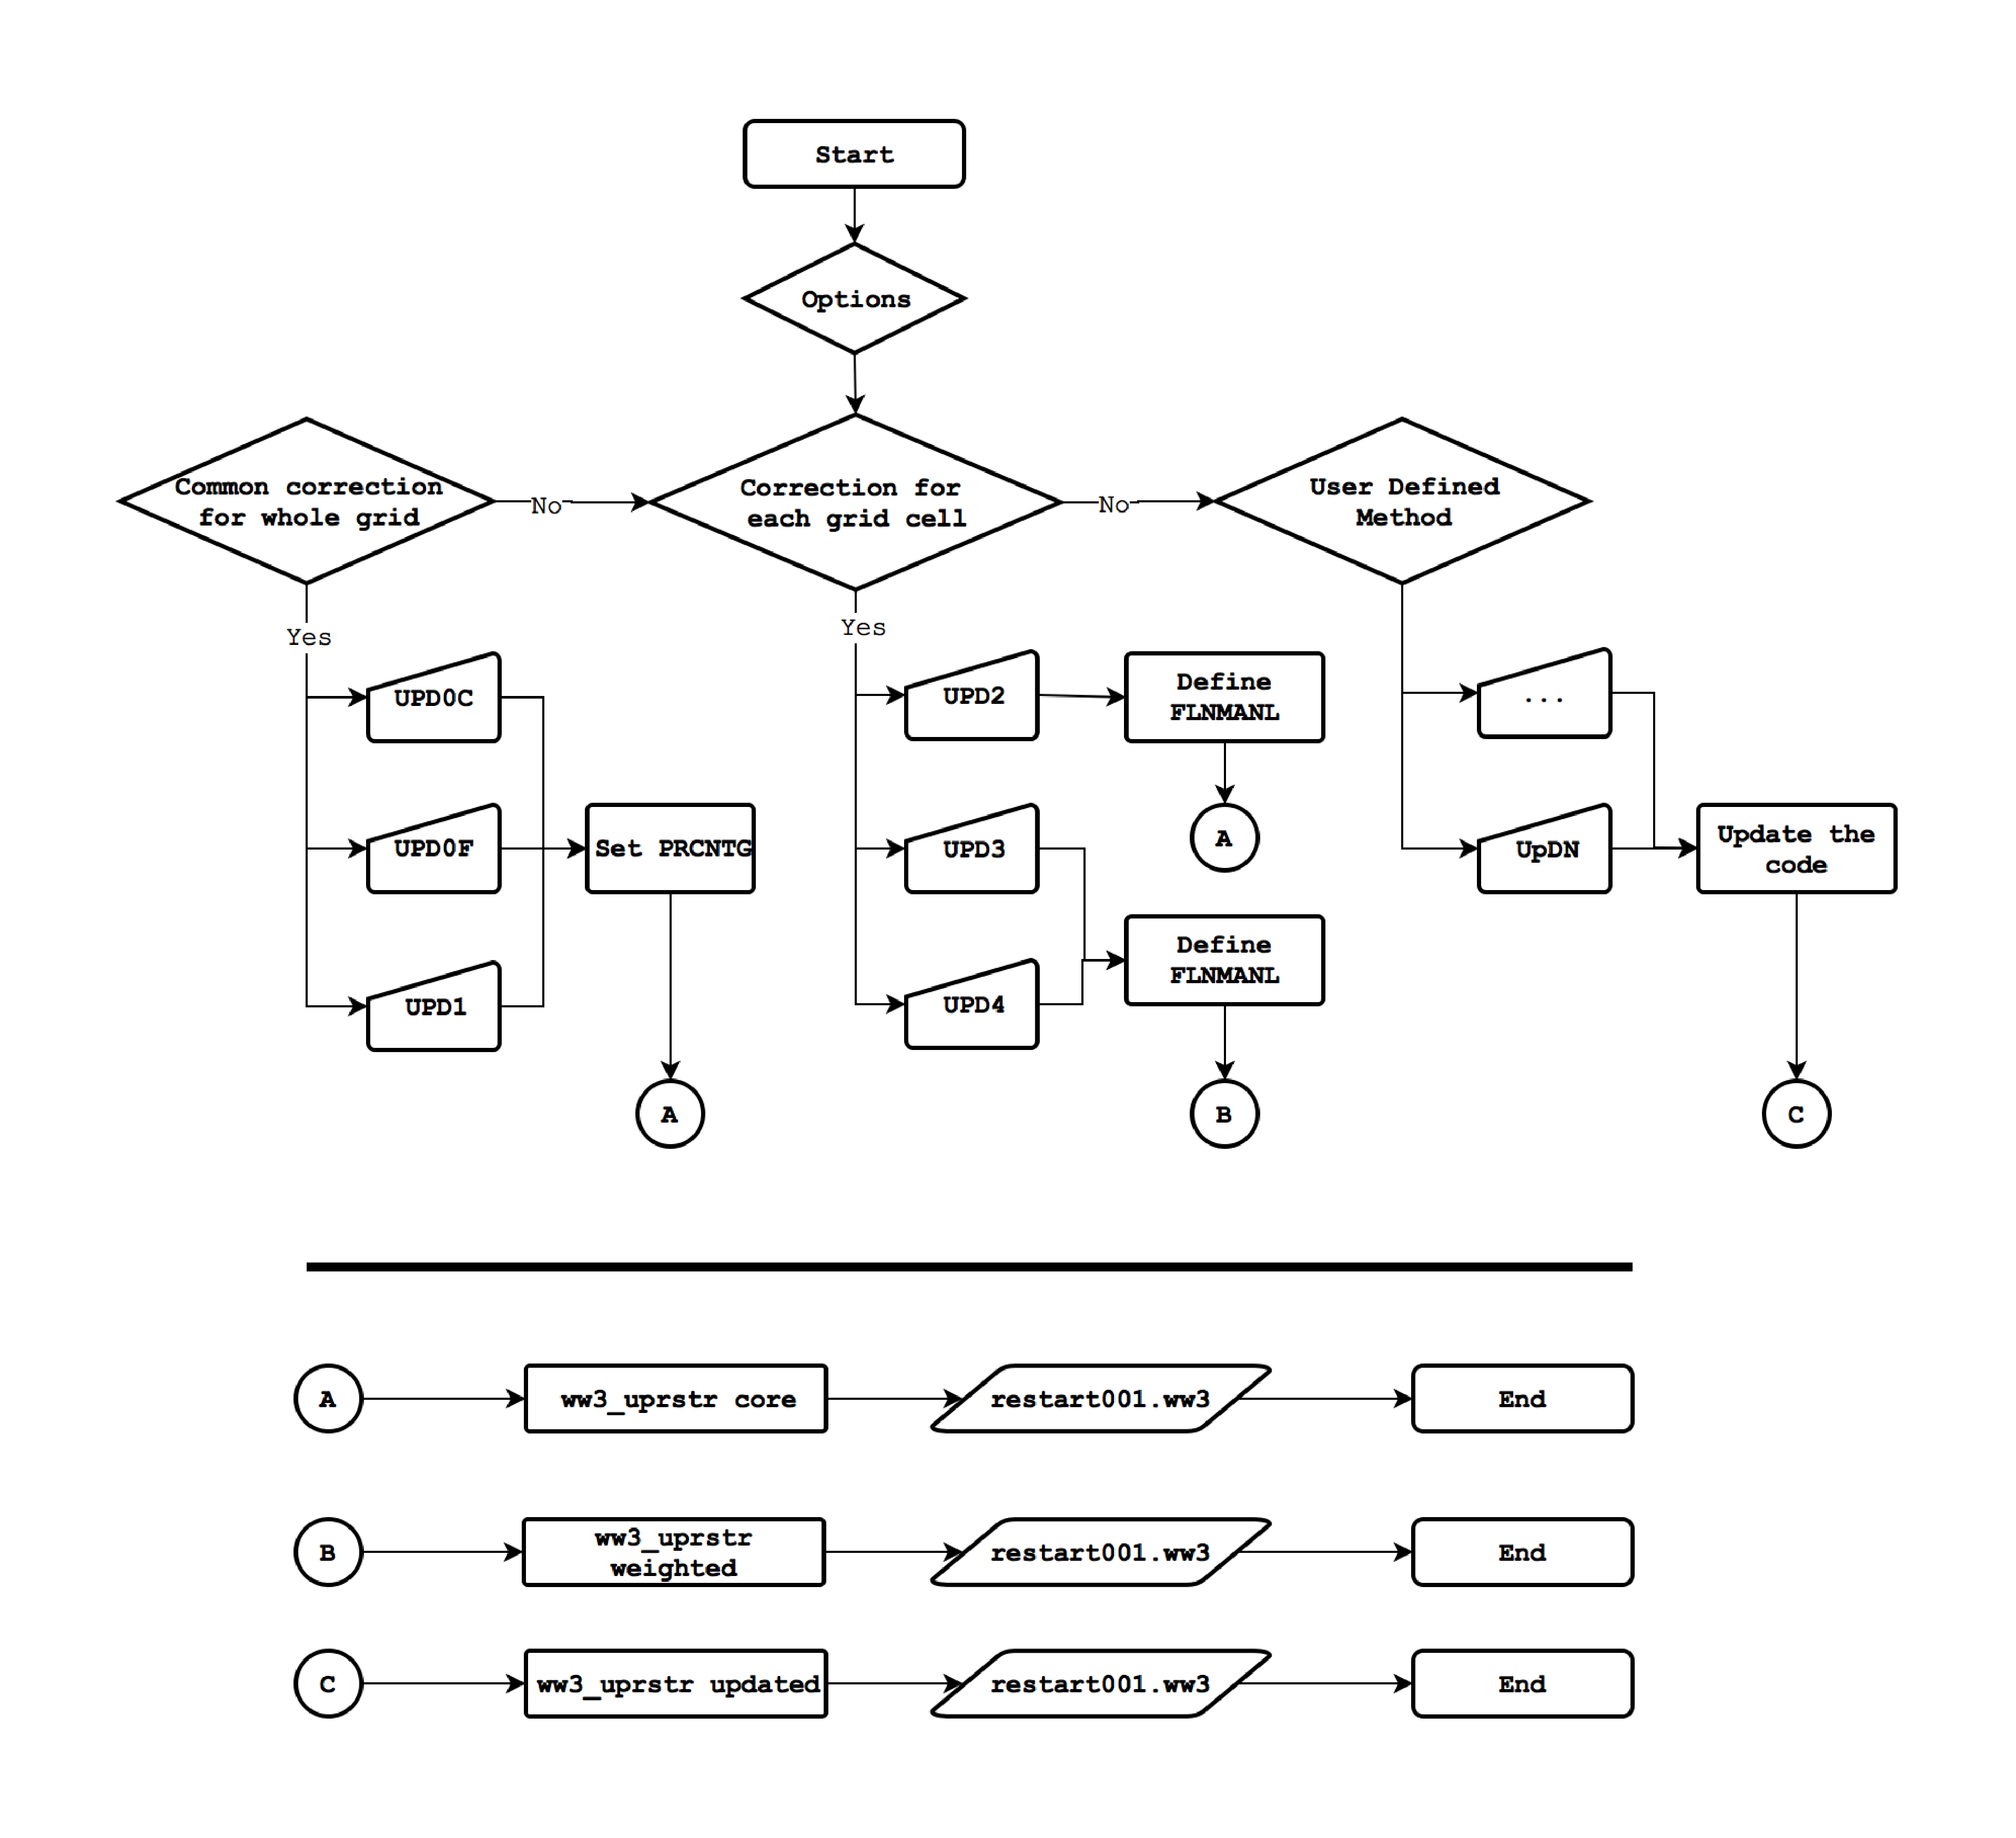
\includegraphics[width=0.9\textwidth]{./run/uprstr.eps}
\caption{Flowchart of the implemented methods for updating the wave spectra at the WW3 
restart file. Additional methods can be implemented by adding UPD options to the namelist.}
\label{fig:uprstrflowchart} \botline
\end{center}
\end{figure}

The following UPD options are available:
\begin{enumerate} 
   \item UPD0C:: \textbf{ELIMINATED from version x.xx} Option 0C  All the spectra are 
   updated with a constant: \newline
      \(fac=(SWH\_Bckg-SWH\_Anl)/SWH\_Anl \).
   \item UPD0F:: Option 0F  All the spectra are updated with a constant: \newline 
      \(fac=SWH\_Anl/SWH\_Bckg \).
   \item UPD1 ::  \textbf{ELIMINATED from version x.xx} Option 1  The fac(x,y,frq,theta), 
   is weighted according to the \% of energy at each spectral bin; fac the same as UPDOF.
   \item UPD2 :: Option 2   The fac(x,y,frq,theta), is calculated at each grid point 
   according to SWH\_Bckg and SWH\_Anl
   \item UPD3 :: Option 3   The update factor is a surface with the shape of 
   the background spectrum. 
   \item UPD4 :: [NOT INCLUDED in the current version, just keeping the spot]
   Option 4  The generalization of the UPD3. The update factor is the sum of surfaces 
   which are applied on the background spectrum. The algorithm requires the mapping 
   of each partition on the individual spectra; the map is used to determine the weighting 
   surfaces.
\end{enumerate}

Any additional method for the redistribution of the energy to the WS could be added 
by extending the input file and adding the source code to the \textbf{ww3\_uprstr.ftn}.

\subparagraph{Example \newline}
In this section, an example of the simplest WDA application is discussed.
The figure ~\ref{fig:waveDAflowchart} shows how the \textbf{ww3\_uprstr} 
is used in the framework of a simple wave analysis system. \newline

A WW3 run (from the previous cycle or from the hindcast) provides the
background field of SWH and the corresponding restart file at the appropriate time. 
The format of the background SWH field has to be compatible with the WDA module inputs.

\begin{figure} \begin{center}
\includegraphics[width=0.9\textwidth]{./run/waveDA.eps}
\caption{Flowchart of simplified wave data assimilation system, 
showing the role of the {ww3\_uprstr}, the required input files,
and the resulted output of the updated restart file.}
\label{fig:waveDAflowchart} \botline
\end{center}
\end{figure}

The WDA module uses the background field and the available observations
for the time of analysis, produces the analysis and exports 
the field of SWH in grbtxt format (\textbf{XXXX.grbtxt}) .

The analysis file, the \textbf{mod\_def.ww3}, the \textbf{restart.ww3} file and 
the \textbf{ww3\_uprstr.inp} are the input files for the \textbf{ww3\_uprstr}. 
If all the options and input files are correctly prepared, it takes approxmately 
one minute to update a grid of 260000 grid nodes and generate the output on a single processor. 
The updated restart file has to be renamed, at the expected file name, in the case of this
example to \textbf{restart.ww3}. \newline  

   \noindent\fbox{
      \parbox{\textwidth}{
      \textbf{Note: }
      All \ncep's WDA systems use GRIB2 format, thereore there is always an intermediate
      step to transfer the grib files to the appropriate format. The used software is WGRIB2 
      and more information can be retrieve from the 
      \href{http://www.cpc.ncep.noaa.gov/products/wesley/wgrib2} {official website}.       
      }
   }

%\paragraph{How to Update the ww3\_uprstr \newline}
%Add data readers, mainly for machine independent binary data and wgrib2.

\pb


% tab:fields

\begin{table} \begin{center}
\begin{tabular}{|c|c|c|c|c|c|} \hline
group & field & description                  &  file        & GRIB1 & GRIB2   \\
      &                              &  extension   & data  & data    \\ \hline \hline
 1 & 1 & depth                           & {\file .dpt} &  --  &    --    \\
 1 & 2 & mean current components         & {\file .cur} &  --  &    --    \\
 1 & 3 & wind speed                      & {\file .wnd} &  32  &  0,2,1   \\
   &&  wind direction                 &              &  31  &  0,2,0   \\
   &&  wind $u$                       &              &  33  &  0,2,2   \\
   &&  wind $v$                       &              &  34  &  0,2,3   \\
 1 & 4 & air-sea temp. dif.              & {\file .dt}  &  --  &    --    \\
 1 & 5 & water level                     & {\file .wlv} &  --  &  10,3,1  \\
 1 & 6 & ice coverage                    & {\file .ice} &  91  &  10,2,0  \\
 2 & 1 & wave height $H_s$               & {\file .hs}  & 100  &  10,0,3  \\
 2 & 2 & mean wave length                & {\file .l}   &  --  &    --    \\
 2 & 3 & mean wave period $T_{m0,2}$     & {\file .t02} &  --  &    --    \\
 2 & 4 & mean wave period $T_{m0,1}$     & {\file .t}   & 103  &  10,0,15 \\
 2 & 5 & mean wave period $T_{m0,-1}$    & {\file .tm1} &  --  &    --    \\
 2 & 6 & peak frequency $f_p$            & {\file .fp}  & 108  &  10,0,11 \\
 2 & 7 & mean wave direction $\theta_m$  & {\file .dir} & 101  &    --    \\
 2 & 8 & directional spread $\sigma$     & {\file .spr} &  --  &    --    \\
 2 & 9 & peak direction $\theta_p$       & {\file .dp}  & 107  &  10,0,10 \\
 4 & 1 & $H_s$ of partition              & {\file .phs} & 102,105 & 10,0,5/8 \\
 4 & 2 & $T_p$ of partition              & {\file .ptp} & 110,106 & 10,0,6/9\\
 4 & 3 & $L_p$ of partition              & {\file .plp} &  --  &    --    \\
 4 & 4 & $\theta_m$ of partition         & {\file .pdir} & 109,104 & 10,0,4/7 \\
 4 & 5 & $\sigma$ of partition           & {\file .psi} &  --  &    --    \\
 4 & 6 & wind sea fraction of part.      & {\file .pws} &  --  &    --    \\
 4 & 7 & total wind sea fraction         & {\file .wsf} &  --  &    --    \\
 4 & 8 & number of partitions            & {\file .pnr} &  --  &    --    \\
 5 & 1 & friction velocity comp.         & {\file .ust} &  --  &    --    \\
 5 & 2 & Charnock par for air side & {\file .cha} &  --  &    --    \\
 5 & 3 & Energy flux $\int C_g E(f) df$  & {\file .CgE} &  --  &    --    \\
 5 & 4 & Wind to wave energy flux        & {\file .faw} &  --  &    --    \\
 5 & 5 & Wave-supported stress           & {\file .taw} &  --  &    --    \\
 5 & 6 & Upward wave-supported stress    & {\file .twa} &  --  &    --    \\
 5 & 7 & Whitecap coeverage              & {\file .wcc} &  --  &    --    \\
 5 & 8 & Avg whitecap foam thickness & {\file .wcf} &  --  &    --    \\
 5 & 9 & Sign breaking wave height& {\file .wch} &  --  &    --    \\
 5 & 10 & Whitecap moment                 & {\file .wcm} &  --  &    --    \\ \hline
\end{tabular} \end{center}
\caption{~Field output post processors ancillary data.} \label{tab:fields}
\vspace{0.5in}
\end{table}

\begin{table} \begin{center}
\begin{tabular}{|c|c|c|c|c|c|} \hline
group & field & description                  &  file        & GRIB1 & GRIB2   \\
      &                              &  extension   & data  & data    \\ \hline \hline
 6 & 1 & radiation stress                & {\file .Sxy} &  --  &    --    \\
 6 & 2 & Breaking wave momentum flux     & {\file .two} &  --  &    --    \\
 6 & 3 & Bernoulli head                  & {\file .J} &  --  &    --    \\
 6 & 4 & Breaking wave energy flux       & {\file .foc} &  --  &    --    \\
 6 & 5 & Stokes transport                & {\file .tus} &  --  &    --    \\
 6 & 6 & Surface Stokes drift            & {\file .uss} &  --  &    --    \\
 6 & 7 & Second order pressure at $k=0$  & {\file .p2s} &  --  &    --    \\
 7 & 1 & near-bottom amplitude           & {\file .cfd} &  --  &    --    \\
 7 & 2 & near-bottom velocity            & {\file .ubr} &  --  &    --    \\
 7 & 3 & bedform parameters              & {\file .bed} &  --  &    --    \\
 7 & 4 & Energy flx to bot bound layer & {\file .fbb} &  --  &    --    \\
 7 & 5 & Momentum flx to bot bound layer & {\file .tbb} &  --  &    --    \\
 8 & 1& mean square slopes              & {\file .mss} &  --  &    --    \\
 8 & 2 & Phillips constant               & {\file .msc} &  --  &    --    \\
 9 & 1 & average time step               & {\file .dtd} &  --  &    --    \\
 9 & 2 & cut-off frequency $f_c$         & {\file .fc}  &  --  &    --    \\
 9 & 3 & cut-off frequency $f_c$         & {\file .fc}  &  --  &    --    \\
 9 & 4 & maximum CFL for X-Y advection   & {\file .cfx} &  --  &    --    \\
 9 & 5 & maximum CFL for $\theta$ advection & {\file .cfd} &  --  &    --    \\
 9 & 6 & maximum CFL for $k$ advection   & {\file .cfk} &  --  &    --    \\
 10 & 1 & user defined \#1                & {\file .us1} &  --  &    --    \\
 10 & 2 & user defined \#2                & {\file .us2} &  --  &    --    \\ \hline
%13 & wind sea period $T_w$           & {\file .fpl} & 110  &    --    \\
%14 & wind sea direction $\theta_w$   & {\file .dpl} & 109  &    --    \\

\end{tabular} \end{center}
\caption*{Table~\ref{tab:fields}, continued.} 
\vspace{0.5in}
\end{table}

\clearpage

%\bpage
